%% Report for RDS 26/27 -- Project 1 (Byzantine fault-tolerant payment service)
%% Based on the ACM `acmart' template (sigconf), as provided by the teacher.
%%
%% Placeholders: everything that still needs your implementation / results is
%% marked with \todo{...} and shown in red in the PDF.  Search for "\todo" to
%% find them all.  When you are done, you can make them disappear (e.g. to
%% check the page count) by changing the definition of \todo below.

\documentclass[sigconf,a4paper]{acmart}

\usepackage{graphicx}
\usepackage{tikz}
\usetikzlibrary{arrows.meta,positioning}

%% ---------------------------------------------------------------------
%% Helper macros
%% ---------------------------------------------------------------------
% Red, bold placeholder.  Use \todo{what has to be written here}.
\newcommand{\todo}[1]{\textcolor{red}{\textbf{[TODO: #1]}}}
% Dashed red box standing in for a figure that still has to be produced.
\newcommand{\figplaceholder}[2]{%
    \fcolorbox{red!70}{red!4}{\parbox[c][#1][c]{\dimexpr\linewidth-2\fboxsep-2\fboxrule\relax}{%
        \centering\small\textcolor{red}{\textbf{[PLACEHOLDER]}}\\#2}}}
% Typesetting of API / message names.
\newcommand{\api}[1]{\texttt{#1}}

%%
%% \BibTeX command to typeset BibTeX logo in the docs
\AtBeginDocument{%
    \providecommand\BibTeX{{%
        \normalfont B\kern-0.5em{\scshape i\kern-0.25em b}\kern-0.8em\TeX}}}

%% Rights management information (SAMPLE values from the template).
\setcopyright{acmcopyright}
\copyrightyear{2026}
\acmYear{2026}
\acmDOI{}

%% Conference information.
\acmConference[RDS 26/27]{Reliable Distributed Systems 2026/27 -- first project}{2026}{Faculdade de Ciências e Tecnologia, NOVA University of Lisbon, Portugal}
\acmBooktitle{Reliable Distributed Systems 2026/27 -- first project, Faculdade de Ciências e Tecnologia, NOVA University of Lisbon, Portugal}
\acmPrice{}
\acmISBN{}

\begin{document}

    \title[Byzantine Fault-Tolerant Payments]{Byzantine Fault-Tolerant Payments: Consensus-free, PBFT and Blockchain Replication}

    \author{António Mendes}
    \authornote{Student number 73530. Blockchain development}
    \email{an.mendes@campus.fct.unl.pt}
    \affiliation{%
        \institution{MEI, DI, FCT, UNL}
    }

    \author{Francisco Almeida}
    \authornote{Student number 75116. BRB and State Machine}
    \email{fs.almeida@campus.fct.unl.pt}
    \affiliation{%
        \institution{MEI, DI, FCT, UNL}
    }

    \author{Bernardo Gracioso}
    \authornote{Student number 75486. PBFT and State Machine}
    \email{b.gracioso@campus.fct.unl.pt}
    \affiliation{%
        \institution{MEI, DI, FCT, UNL}
    }

    \renewcommand{\shortauthors}{António, Francisco, and Bernardo.}

%% ---------------------------------------------------------------------
    \begin{abstract}
        We design, implement and evaluate a replicated payment service that
        tolerates Byzantine faults in both replicas and clients: a (very)
        simplified version of the systems that manage account balances in a bank or
        in a cryptocurrency. The service must guarantee that money is never created
        or destroyed, that only the owners of an account can spend its funds, and
        that the same funds are never spent twice. On top of a fixed application
        layer and the Babel~2 framework, we build three replication solutions with
        different guarantees: consensus-free payments over Byzantine Reliable
        Broadcast, which imposes no total order on transfers; state machine
        replication over PBFT, which yields a consistent total order; and a
        Proof-of-Work blockchain, where blocks of transfers establish a
        tamper-evident and eventually consistent order. We argue the correctness of
        each solution in a partially synchronous system with $n \ge 3f+1$ replicas
        and compare them in terms of throughput, latency and consistency when
        accounts are shared by several owners.
        \todo{aqui resumimos um pouco os resultados}
    \end{abstract}

    \maketitle

%% ---------------------------------------------------------------------
    \section{Introduction}
    \label{sec:intro}

    Systems that manage account balances, such as those of a bank or of a
    cryptocurrency, must remain available and trustworthy even when some of their
    components fail or are compromised. Replicating the service tolerates crashes,
    but when replicas (and clients) can behave arbitrarily, i.e.\ under the
    Byzantine fault model, the replicated service must still ensure that money is
    never created or destroyed, that only the owner of an account can spend its
    funds, and that the same funds are never spent twice (\emph{double spending}).

    This report documents a replicated payment service that lets clients
    transfer funds from an account they own to any other account, read the
    balance of an account, and read the history of transfers (outgoing and
    incoming) of an account.

    It is well known that state machine replication requires consensus to order
    operations. However, a payment system where each account has a \emph{single
    owner} does not need consensus: it is enough that all transfers from the same
    account are executed in the order defined by its owner, and transfers from
    different accounts commute (in the absence of double-spending attempts)
    \cite{the-consensus-number-of-a-cryptocurrency}. This result inspired
    practical systems \cite{online-payments-by-merely-broadcasting-messages}, but
    stops being true as soon as accounts can be shared by several owners. A
    central goal of our work is to observe, explain and measure the consequences
    of this observation.

    To this end, we implemented three replication solutions underneath the same
    application logic, each with distinct guarantees:
    \begin{itemize}
        \item \textbf{Consensus-free payments}, based only on Byzantine Reliable
        Broadcast \cite{asynchronous-byzantine-agreement-protocols,introduction-to-reliable-and-secure-distributed-programming}
        between replicas, without a global (total) order on transfers;
        \item \textbf{PBFT-based payments}, where state machine replication over
        Practical Byzantine Fault Tolerance \cite{practical-byzantine-fault-tolerance}
        provides a consistent total order;
        \item \textbf{Blockchain-based payments}, a replicated blockchain heavily
        inspired by Bitcoin \cite{bitcoin}, where blocks of transfers establish a
        tamper-evident and eventually consistent order.
    \end{itemize}
    All of them are implemented in Java using Babel~2, the evolution of the Babel
    framework \cite{babel_framework}.

    \todo{aqui entramos em mais detalhe sobre o que obtivemos de resultados e assim}

    The remainder of the paper is organized as follows. Section~\ref{sec:background}
    introduces the payment service and the building blocks we rely on;
    Section~\ref{sec:model} states the system model and the threats we consider;
    Section~\ref{sec:impl} describes the architecture and the three solutions;
    Section~\ref{sec:correctness} argues their correctness;
    Section~\ref{sec:eval} presents the experimental evaluation; and
    Section~\ref{sec:conclusion} concludes.

%% ---------------------------------------------------------------------
    \section{Background}
    \label{sec:background}

    \subsection{The Payment Service}

    The service manages a fixed set of \emph{accounts}, each with a name, a
    balance and a set of \emph{owners}. Owners are clients, identified by a public
    key known to all replicas. In the initial state of the system (the
    \emph{genesis}), every client owns an account with its own name, a few
    \emph{shared accounts} are owned by several clients, and all accounts start
    with the same balance.

    A \emph{transfer} is the operation replicated by the system. It is composed of
    $\langle from, to, amount, seq, signer\rangle$ and a signature of the signer
    over these fields. A transfer is \emph{valid} if both accounts exist and are
    different, the amount is positive, the signer is one of the owners of account
    $from$, and the signature is correct. Each account has its own sequence of
    transfers: the transfer of account $A$ with sequence number $s$ can only be
    executed after the transfers of $A$ with sequence numbers $0,1,\ldots,s-1$.
    Two different transfers from the same account with the same sequence number
    are \emph{conflicting}: at most one of them can ever be executed.

    Each replica keeps its state in a deterministic \emph{ledger}. When a valid
    transfer is handed to the ledger, it is either (i) \emph{executed}, if it is
    the next transfer of its account and the account has enough funds (which may
    trigger the execution of other pending transfers); (ii) kept \emph{pending},
    if previous transfers of the account were not executed yet or the account
    lacks funds; or (iii) \emph{rejected as a conflict}, if a different transfer of
    the same account with the same sequence number was handed to the ledger first.
    If every account has a single (correct) owner, the final ledger state does not
    depend on the order in which transfers of different accounts are handed to it;
    with shared accounts, two owners may concurrently issue conflicting transfers,
    and replicas that see them in different orders diverge.

    \paragraph{Clients.} Since replicas may be Byzantine, a client cannot trust the
    reply of a single replica (Figure~\ref{fig:client}): it sends each request to
    all replicas and accepts a result only after receiving $f+1$ matching replies
    from different replicas, which ensures that at least one correct replica
    vouches for it. Replicas reply to a transfer once its outcome is known
    (executed, invalid, or conflicting), while balance and history requests are
    answered immediately from the replica's local state. To issue a transfer, a
    client must know the next sequence number of the account: for its own account
    it simply keeps track of it, while for a shared account it must first read it
    with a balance request, and other owners may be doing the same concurrently.

    \begin{figure}[t]
        \centering
        \resizebox{\linewidth}{!}{%
            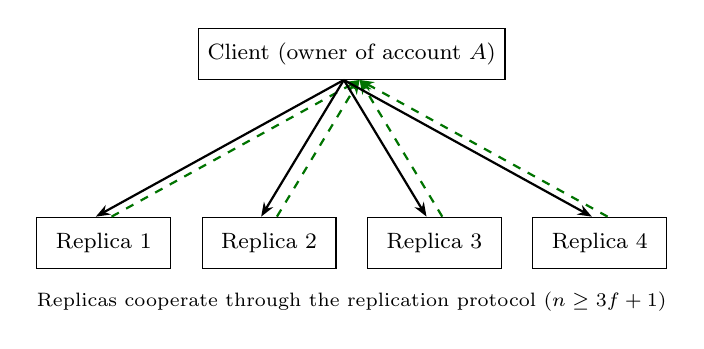
\begin{tikzpicture}[
                box/.style={draw, minimum width=1.7cm, minimum height=0.65cm, font=\footnotesize, align=center},
                req/.style={-{Stealth[length=1.8mm]}, thick},
                rep/.style={-{Stealth[length=1.8mm]}, thick, dashed, green!45!black}
            ]
                \node[box, minimum width=3cm] (c) at (3.15,2.4) {Client (owner of account $A$)};
                \foreach \i/\x in {1/0, 2/2.1, 3/4.2, 4/6.3} {
                    \node[box] (r\i) at (\x,0) {Replica \i};
                    \draw[req] ([xshift=-1mm]c.south) -- ([xshift=-1mm]r\i.north);
                    \draw[rep] ([xshift=1mm]r\i.north) -- ([xshift=1mm]c.south);
                }
                \node[font=\scriptsize] at (3.15,-0.75) {Replicas cooperate through the replication protocol ($n\ge 3f+1$)};
            \end{tikzpicture}}
        \caption{Interaction between a client and the replicas. Solid arrows: the
        signed request is sent to all replicas. Dashed arrows: replies; the result
        is accepted after $f+1$ matching ones.}
        \Description{A client sends a request to four replicas and accepts the result after f+1 matching replies.}
        \label{fig:client}
    \end{figure}

    \subsection{Building Blocks}

    \paragraph{Byzantine Reliable Broadcast (BRB).} BRB
    \cite{asynchronous-byzantine-agreement-protocols,introduction-to-reliable-and-secure-distributed-programming}
    lets a process request the broadcast of a message
    (\api{brbBroadcast(m)}) and notifies the delivery of messages
    (\api{brbDeliver(p, m)}) such that, even if the sender is Byzantine, all
    correct processes deliver the same message for a given broadcast instance
    (\emph{consistency}), if one correct process delivers a message then all
    correct processes eventually do (\emph{totality}), and a message broadcast by
    a correct process is eventually delivered by all correct processes
    (\emph{validity}). BRB does \emph{not} order messages from different
    instances.

    \paragraph{PBFT.} Practical Byzantine Fault Tolerance
    \cite{practical-byzantine-fault-tolerance} implements state machine
    replication with $n \ge 3f+1$ replicas, $f$ of which may be Byzantine. In each
    view, a primary assigns sequence numbers to (batches of) requests through the
    pre-prepare, prepare and commit phases; checkpoints bound the log; and a view
    change replaces a primary suspected to be faulty. Safety holds in asynchronous
    systems, and liveness requires partial synchrony. In this project the
    membership is static, so a view change only replaces the primary.

    \paragraph{Proof-of-Work blockchains.} In Bitcoin-style systems
    \cite{bitcoin}, transfers are grouped into blocks; each block references the
    hash of the previous block, forming a chain, and includes a proof-of-work (a
    nonce such that the hash of the block has a given number of leading zeros).
    Participants adopt the longest valid chain. A block is considered stable once
    it has $k$ confirmations, so consistency is eventual and, in general,
    probabilistic.

    \subsection{Babel 2}

    We use Babel~2, the evolution of the Babel framework \cite{babel_framework}
    developed in the NOVA LINCS laboratory. Protocols are event-driven state
    machines written in Java, declaring their handlers through annotations;
    messages are Java records whose serializers are generated automatically; and
    requests and indications between protocols of the same process are events.
    Inter-process communication relies on the Netty framework, which the
    framework hides from the programmer. Channels authenticate the identity of the
    other side when a connection is established, and a message is delivered to
    \emph{every} protocol that handles its type, independently of the channel
    where it was received.

%% ---------------------------------------------------------------------
    \section{System Model and Threats}
    \label{sec:model}

    We consider a partially synchronous system under the Byzantine fault model,
    with a static set of $n \ge 3f+1$ replicas, of which at most $f$ can be
    Byzantine. Any number of clients can be Byzantine, but a correct client never
    discloses its private key. Processes communicate through authenticated perfect
    point-to-point links: the channels provided by Babel~2 verify the identity of
    the other side when a connection is established, so the sender of every
    message is authenticated. Whenever a process must convince a third party that
    some process said something (e.g., to build certificates in PBFT), messages
    must be explicitly signed. Cryptographic primitives cannot be broken.

    Table~\ref{tab:threats} lists the attacks we considered and how each one is
    handled (or mitigated) by our solutions.

    \begin{table}[t]
        \centering
        \small
        \caption{Threats considered and how they are handled.}
        \label{tab:threats}
        \begin{tabular}{p{3.35cm}p{4.25cm}}
            \toprule
            \textbf{Threat} & \textbf{Handling / mitigation} \\
            \midrule
            Clients issuing transfers from accounts they do not own, or replaying or tampering with transfers of others
            & Transfers are signed by their signer and checked against the owners of $from$; the sequence number makes a replayed transfer a duplicate. \todo{confirmar onde cada check é feito em cada solução} \\
            \addlinespace
            Clients (or replicas) double spending, e.g.\ two conflicting transfers sent to different replicas
            & \todo{para cada : BRB / PBFT / blockchain} \\
            \addlinespace
            Byzantine replicas that equivocate, omit messages or relay messages to only some replicas
            & \todo{BRB} \\
            \addlinespace
            Byzantine primary that does not order (some) transfers, or proposes invalid, duplicated or different batches
            & \todo{PBFT} \\
            \addlinespace
            Byzantine miners that withhold blocks, disseminate invalid blocks or try to rewrite the chain
            & \todo{blockchain} \\
            \addlinespace
            Processes that are not replicas sending replica-to-replica messages
            & \todo{verificar sender} \\
            \bottomrule
        \end{tabular}
    \end{table}

%% ---------------------------------------------------------------------
    \section{Architecture and Implementation}
    \label{sec:impl}

    \subsection{Layering}

    Each replica is composed of three layers (Figure~\ref{fig:arch}): the
    \emph{payment service} (application logic, provided); a \emph{replication
    protocol} (simple replication, state machine replication, or blockchain); and
    a \emph{dissemination/agreement protocol} (Byzantine Reliable Broadcast or
    PBFT). The BRB protocol is used by two of the alternatives, so it is
    implemented once and reused. The interfaces between layers are:
    \begin{itemize}
        \item payment service $\leftrightarrow$ replication protocol (all variants):
        request \api{SubmitTransaction(tx)} and indication
        \api{ExecuteTransaction(tx)}, which hands one transfer at a time to the
        ledger, in the order in which it must be executed;
        \item replication protocol $\leftrightarrow$ BRB: request
        \api{brbBroadcast(m)} and indication \api{brbDeliver(p, m)};
        \item state machine replication $\leftrightarrow$ PBFT: requests
        \api{Propose(batch)} and \api{SuspectPrimary(view)}, and indications
        \api{Decided(sqn, batch)} (in sequence number order, without gaps) and
        \api{ViewChanged(view, primary)}.
    \end{itemize}

    \begin{figure*}[t]
        \centering
        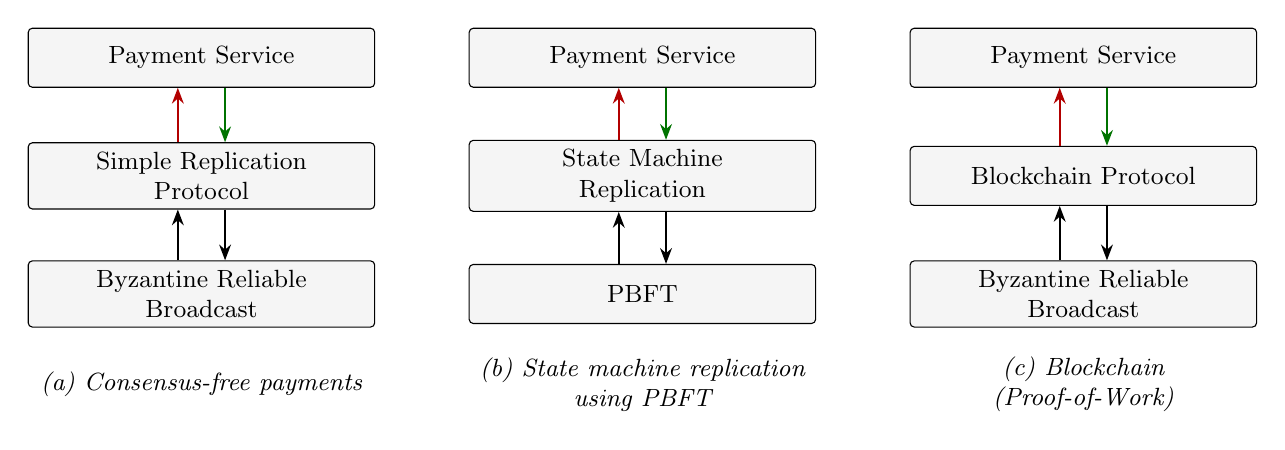
\begin{tikzpicture}[
            layer/.style={draw, rounded corners=1.5pt, minimum width=4.4cm, minimum height=0.75cm, align=center, font=\small, fill=black!4},
            up/.style={-{Stealth[length=2mm]}, thick, red!70!black},
            down/.style={-{Stealth[length=2mm]}, thick, green!45!black},
            both/.style={-{Stealth[length=2mm]}, thick}
        ]
            \newcommand{\replicastack}[4]{%
                \begin{scope}[xshift=#1]
                \node[layer] (ps) at (0,3.0) {Payment Service};
                \node[layer] (rp) at (0,1.5) {#2};
                \node[layer] (dp) at (0,0)   {#3};
                \draw[up]   ([xshift=-3mm]rp.north) -- ([xshift=-3mm]ps.south);
                \draw[down] ([xshift=3mm]ps.south)  -- ([xshift=3mm]rp.north);
                \draw[both] ([xshift=-3mm]dp.north) -- ([xshift=-3mm]rp.south);
                \draw[both] ([xshift=3mm]rp.south)  -- ([xshift=3mm]dp.north);
                \node[font=\small\itshape, align=center] at (0,-1.15) {#4};
                \end{scope}}
            \replicastack{0cm}{Simple Replication\\Protocol}{Byzantine Reliable\\Broadcast}{(a) Consensus-free payments}
            \replicastack{5.6cm}{State Machine\\Replication}{PBFT}{(b) State machine replication\\using PBFT}
            \replicastack{11.2cm}{Blockchain Protocol}{Byzantine Reliable\\Broadcast}{(c) Blockchain\\(Proof-of-Work)}
        \end{tikzpicture}
        \caption{Architecture of a replica and its three variants. Between the
        payment service and the replication protocol, the red upward arrow is the
        \api{ExecuteTransaction} indication and the green downward arrow is the
        \api{SubmitTransaction} request; the black arrows are the requests and
        indications of the dissemination/agreement layer.}
        \Description{Three layered stacks: payment service on top, a replication protocol in the middle and BRB or PBFT at the bottom.}
        \label{fig:arch}
    \end{figure*}

    \subsection{Application Layer}

    The application layer (payment service and ledger) is provided and shared by
    the three solutions. When a replica receives a valid transfer from a client, it
    submits it to the replication protocol, and hands it to the ledger only when
    the replication protocol indicates that it should be executed. As clients send
    their requests to all replicas, the same transfer is typically submitted by
    several replicas, and a Byzantine replica or client might submit anything,
    including old or invalid transfers. The ledger ignores duplicates, but the
    replication protocols should avoid wasting resources disseminating or ordering
    the same transfer several times. The application submits each transfer only
    \emph{once}, so it is the replication protocol's responsibility to ensure that
    every submitted transfer is eventually executed (e.g., even across view
    changes). Periodically, the application logs a digest of its state (balances,
    next sequence numbers and executed transfers of every account): correct
    replicas that executed the same transfers have the same digest, regardless of
    the order, which we use to check whether they converged.

    \subsection{Byzantine Reliable Broadcast}

    \todo{resumir uma beca a cena do echo e dos passos bla bla}

    \subsection{Consensus-free Payments}

    In this variant the replication protocol has almost no logic of its own:
    transfers submitted by the application are handed to BRB, and the replication
    protocol hands them to the application as soon as they are delivered. Correct
    replicas eventually deliver the same set of transfers, but no global order is
    guaranteed.

    \todo{explicar como duas mensagens diferentes não podem ser elivered por dois processos corretos na mesma ronda... como cenas duplicadas vão de vela, etc... outras cenas de estado do protocolo}

    \subsection{State Machine Replication over PBFT}

    In this variant the replication protocol is a state machine replication layer
    on top of PBFT. The primary groups transfers into batches and proposes them to
    PBFT, which establishes a consistent total order; decided batches are executed
    in sequence number order. When the primary is replaced, pending transfers must
    not be lost, but eventually ordered and executed: replicas forward transfers
    to the primary and suspect it (\api{SuspectPrimary}) when transfers are not
    ordered in due time. Every PBFT message (pre-prepare, prepare, commit,
    checkpoint, view-change and new-view) is digitally signed by its sender; the
    MAC/authenticator optimizations of the original paper are not used.

    \todo{Batching (tamanho e timeout), request forwarding e suspeita de
    timeouts, checkpoint e garbage-collection?, view-change e nova-view,
    duplicados, SMR e PBFT (separation of concerns).}

    \subsection{Blockchain}

    In this variant the replication protocol groups transfers into blocks. Each
    block references the hash of the previous block and includes a proof-of-work: a
    nonce such that the hash of the block has a configurable number of leading
    zeros. Replicas act as miners and disseminate the blocks they mine through BRB.
    Each replica validates the blocks it receives, manages its local view of the
    chain, and adopts the longest valid chain. Once a block is $k$ blocks deep
    ($k$ is a parameter), its transfers are considered stable and are handed to the
    application, which never rolls a transfer back; hence a transfer is executed
    only after $k$ blocks were appended after the block that includes it.

    \todo{formato e tamanho, pending-transfer pool, mining loop e
    difficulty, validacao de blocos, fork handling, e valores de $k$ e de dificuldade.}

%% ---------------------------------------------------------------------
    \section{Correctness}
    \label{sec:correctness}

    For each alternative, we argue why correct replicas never execute an invalid
    transfer, why money is never created or destroyed, and why there is no double
    spending (or, when that is not the case, under which conditions it can
    happen and why), in a partially synchronous system under the Byzantine fault
    model.

    \subsection{Common Ground}

    \todo{Arguments that hold for the three solutions because they come from the
    provided application layer: validity checks (signature, owner of $from$, existing
    and distinct accounts, positive amount), per-account sequence numbers,
        conflict rejection and the conservation of the total amount by every executed
        transfer. State precisely what is the ledger's responsibility and what is the
        replication protocol's.}

    \subsection{Consensus-free Payments}

    \todo{Safety (consistency of BRB, why two conflicting transfers cannot both be
    executed by correct replicas for single-owner accounts), liveness (why every
    transfer of a correct client is eventually executed, i.e.\ why $n \ge 3f+1$ and
    partial synchrony suffice), and what can go wrong with shared accounts.}

    \subsection{PBFT-based Payments}

    \todo{Agreement and total order (quorum intersection with $n \ge 3f+1$),
        preservation of decided batches across view changes, why a Byzantine primary
        cannot make correct replicas execute an invalid, duplicated or inconsistent
        batch, and liveness (view change with partial synchrony).}

    \subsection{Blockchain-based Payments}

    \todo{Why invalid blocks are never adopted, why executing a transfer only after
        $k$ confirmations bounds the chance of a rollback, under which conditions (an
        adversary rewriting more than $k$ blocks, e.g.\ the adversary's share of the
        mining power) double spending can still happen, and what happens with transfers
        in blocks that are abandoned.}

%% ---------------------------------------------------------------------
    \section{Experimental Evaluation}
    \label{sec:eval}

    \subsection{Setup}

    \todo{Infrastructure (DI/NOVA LINCS cluster or the alternative announced on
    clip): machines, how replicas and clients are distributed across them, $n$ and $f$, JVM and
    software versions, and how experiments are automated.}
% ver do cluster

    Load is generated by the provided client, which emulates several logical
    clients in a closed loop: each executes one operation at a time, either a
    transfer from its own account, a transfer from a shared account it owns (after
    reading the next sequence number of the account), or a read of a balance or of
    the history of a random account. Each run has a preparation phase (to
    establish connections), a measurement period and a cooldown. The client
    reports the throughput (operations completed per second) and the latency
    (average, median, 95th and 99th percentiles) of each type of operation, the
    number of failed operations (e.g., conflicting transfers), of operations that
    timed out, and of requests for which replicas sent divergent replies, along
    with the number of operations completed in each second. At the end of every
    run we also collect the final state digest of each replica.
    Table~\ref{tab:params} lists the client parameters.

    \begin{table}[t]
        \centering
        \small
        \caption{Client parameters: defaults of the base code and the values used in our experiments.}
        \label{tab:params}
        \begin{tabular}{lrr}
            \toprule
            \textbf{Property} & \textbf{Default} & \textbf{Used} \\
            \midrule
            \texttt{num\_clients}         & 10    & \todo{} \\
            \texttt{transfer\_percentage} & 80    & \todo{} \\
            \texttt{history\_percentage}  & 0     & \todo{} \\
            \texttt{shared\_percentage}   & 0     & \todo{} \\
            \texttt{max\_amount}          & 10    & \todo{} \\
            \texttt{reply\_quorum}        & $f+1$ & \todo{} \\
            \texttt{operation\_timeout}   & 5000\,ms  & \todo{} \\
            \texttt{prepare\_time}        & 3000\,ms  & \todo{} \\
            \texttt{run\_time}            & 30000\,ms & \todo{} \\
            \texttt{cooldown\_time}       & 5000\,ms  & \todo{} \\
            \bottomrule
        \end{tabular}
    \end{table}

    We evaluate the three solutions on the following aspects:
    \begin{itemize}
        \item \textbf{Throughput}: number of operations (in particular transfers)
        executed per unit of time, as the number of clients grows, and also with the
        number of replicas, the size of batches and blocks, or under disruptions;
        \item \textbf{Latency}: time for a transfer to be executed in a
        non-reversible way, i.e.\ for the client to gather $f+1$ matching replies,
        and how it evolves with load, number of replicas, depth $k$ in the
        blockchain, or disruptions;
        \item \textbf{Consistency}: the consequences of the absence of total order,
        namely what happens when clients use shared accounts with each alternative
        (fraction of conflicting transfers, and whether correct replicas converge to
        the same state).
    \end{itemize}
    \todo{List the experiments actually run and the parameter values: number of
    clients, $n$ (e.g.\ 4, 7, 10), batch/block size, block difficulty and $k$,
        percentage of shared-account transfers, crash of a replica, number of
        repetitions per configuration.}

    \subsection{Throughput}

    \begin{figure}[t]
        \centering
        \figplaceholder{3.6cm}{Throughput (ops/s) vs.\ number of clients, one line per solution}
        \caption{\todo{throughput of each solution as the number of clients grows}}
        \Description{Placeholder for a throughput plot.}
        \label{fig:throughput}
    \end{figure}

    \todo{Discuss Figure~\ref{fig:throughput}: saturation points, how the three
    solutions compare, and why (message complexity of BRB and PBFT, batching,
        proof-of-work difficulty and block size, confirmation depth). Include the
        effect of the number of replicas, batch/block size, and of a disruption such as
        the crash of a replica (using the per-second operation counts).}

    \subsection{Latency}

    \begin{figure}[t]
        \centering
        \figplaceholder{3.6cm}{Latency (avg, median, p95, p99) per solution and load}
        \caption{\todo{latency of transfers for each solution}}
        \Description{Placeholder for a latency plot.}
        \label{fig:latency}
    \end{figure}

    \todo{Discuss Figure~\ref{fig:latency}: latency vs.\ load, number of replicas
    and depth $k$; the tail (p95/p99); cost of a view change or of a fork.}

    \subsection{Consistency}

    Without a total order, replicas may report different balances or histories for
    the same account at a given moment, and the client might not gather $f+1$
    matching replies. This is expected, and we quantify it with the number of
    requests with divergent replies and of failed (conflicting) transfers.

    \begin{table}[t]
        \centering
        \small
        \caption{Behaviour with shared accounts (\todo{percentage of shared-account transfers}).}
        \label{tab:consistency}
        \begin{tabular}{lrrr}
            \toprule
            \textbf{Solution} & \textbf{Conflicts} & \textbf{Divergent} & \textbf{Digests} \\
            & \textbf{(\%)} & \textbf{replies (\%)} & \textbf{equal?} \\
            \midrule
            Consensus-free & \todo{} & \todo{} & \todo{} \\
            PBFT           & \todo{} & \todo{} & \todo{} \\
            Blockchain     & \todo{} & \todo{} & \todo{} \\
            \bottomrule
        \end{tabular}
    \end{table}

    \todo{Discuss Table~\ref{tab:consistency}: whether correct replicas converge
    to the same state (compare digests) with and without shared accounts for each
    alternative, and why.}

    \subsection{Discussion}

    \todo{Trade-offs among the three solutions (guarantees vs.\ performance),
        when each one is preferable, and limitations of the evaluation.}

%% ---------------------------------------------------------------------
    \section{Conclusion}
    \label{sec:conclusion}

    We implemented a Byzantine fault-tolerant replicated payment service in three
    ways, with no total order (BRB), with a total order (PBFT), and with an
    eventually consistent order (Proof-of-Work blockchain), over the same
    application logic and the Babel~2 framework.
    \todo{resumir os resultados e coisas a notar e pronto ig}

%%
%% Bibliography
    \bibliographystyle{ACM-Reference-Format}
    \bibliography{references}

\end{document}
\endinput